\chapter{Einleitung} \label{chap:Einleitung}
\thispagestyle{empty}
Gesetzliche Bestimmungen zur Erhöhung der Sicherheit von sowohl den Insassen eines Fahrzeugs als auch anderer Verkehrsteilnehmer haben in den letzten Jahrzehnten zu einer signifikanten Senkung der Mortalitätsrate bei Verkehrsunfällen beigetragen.
\begin{figure}[H]
    \centering
    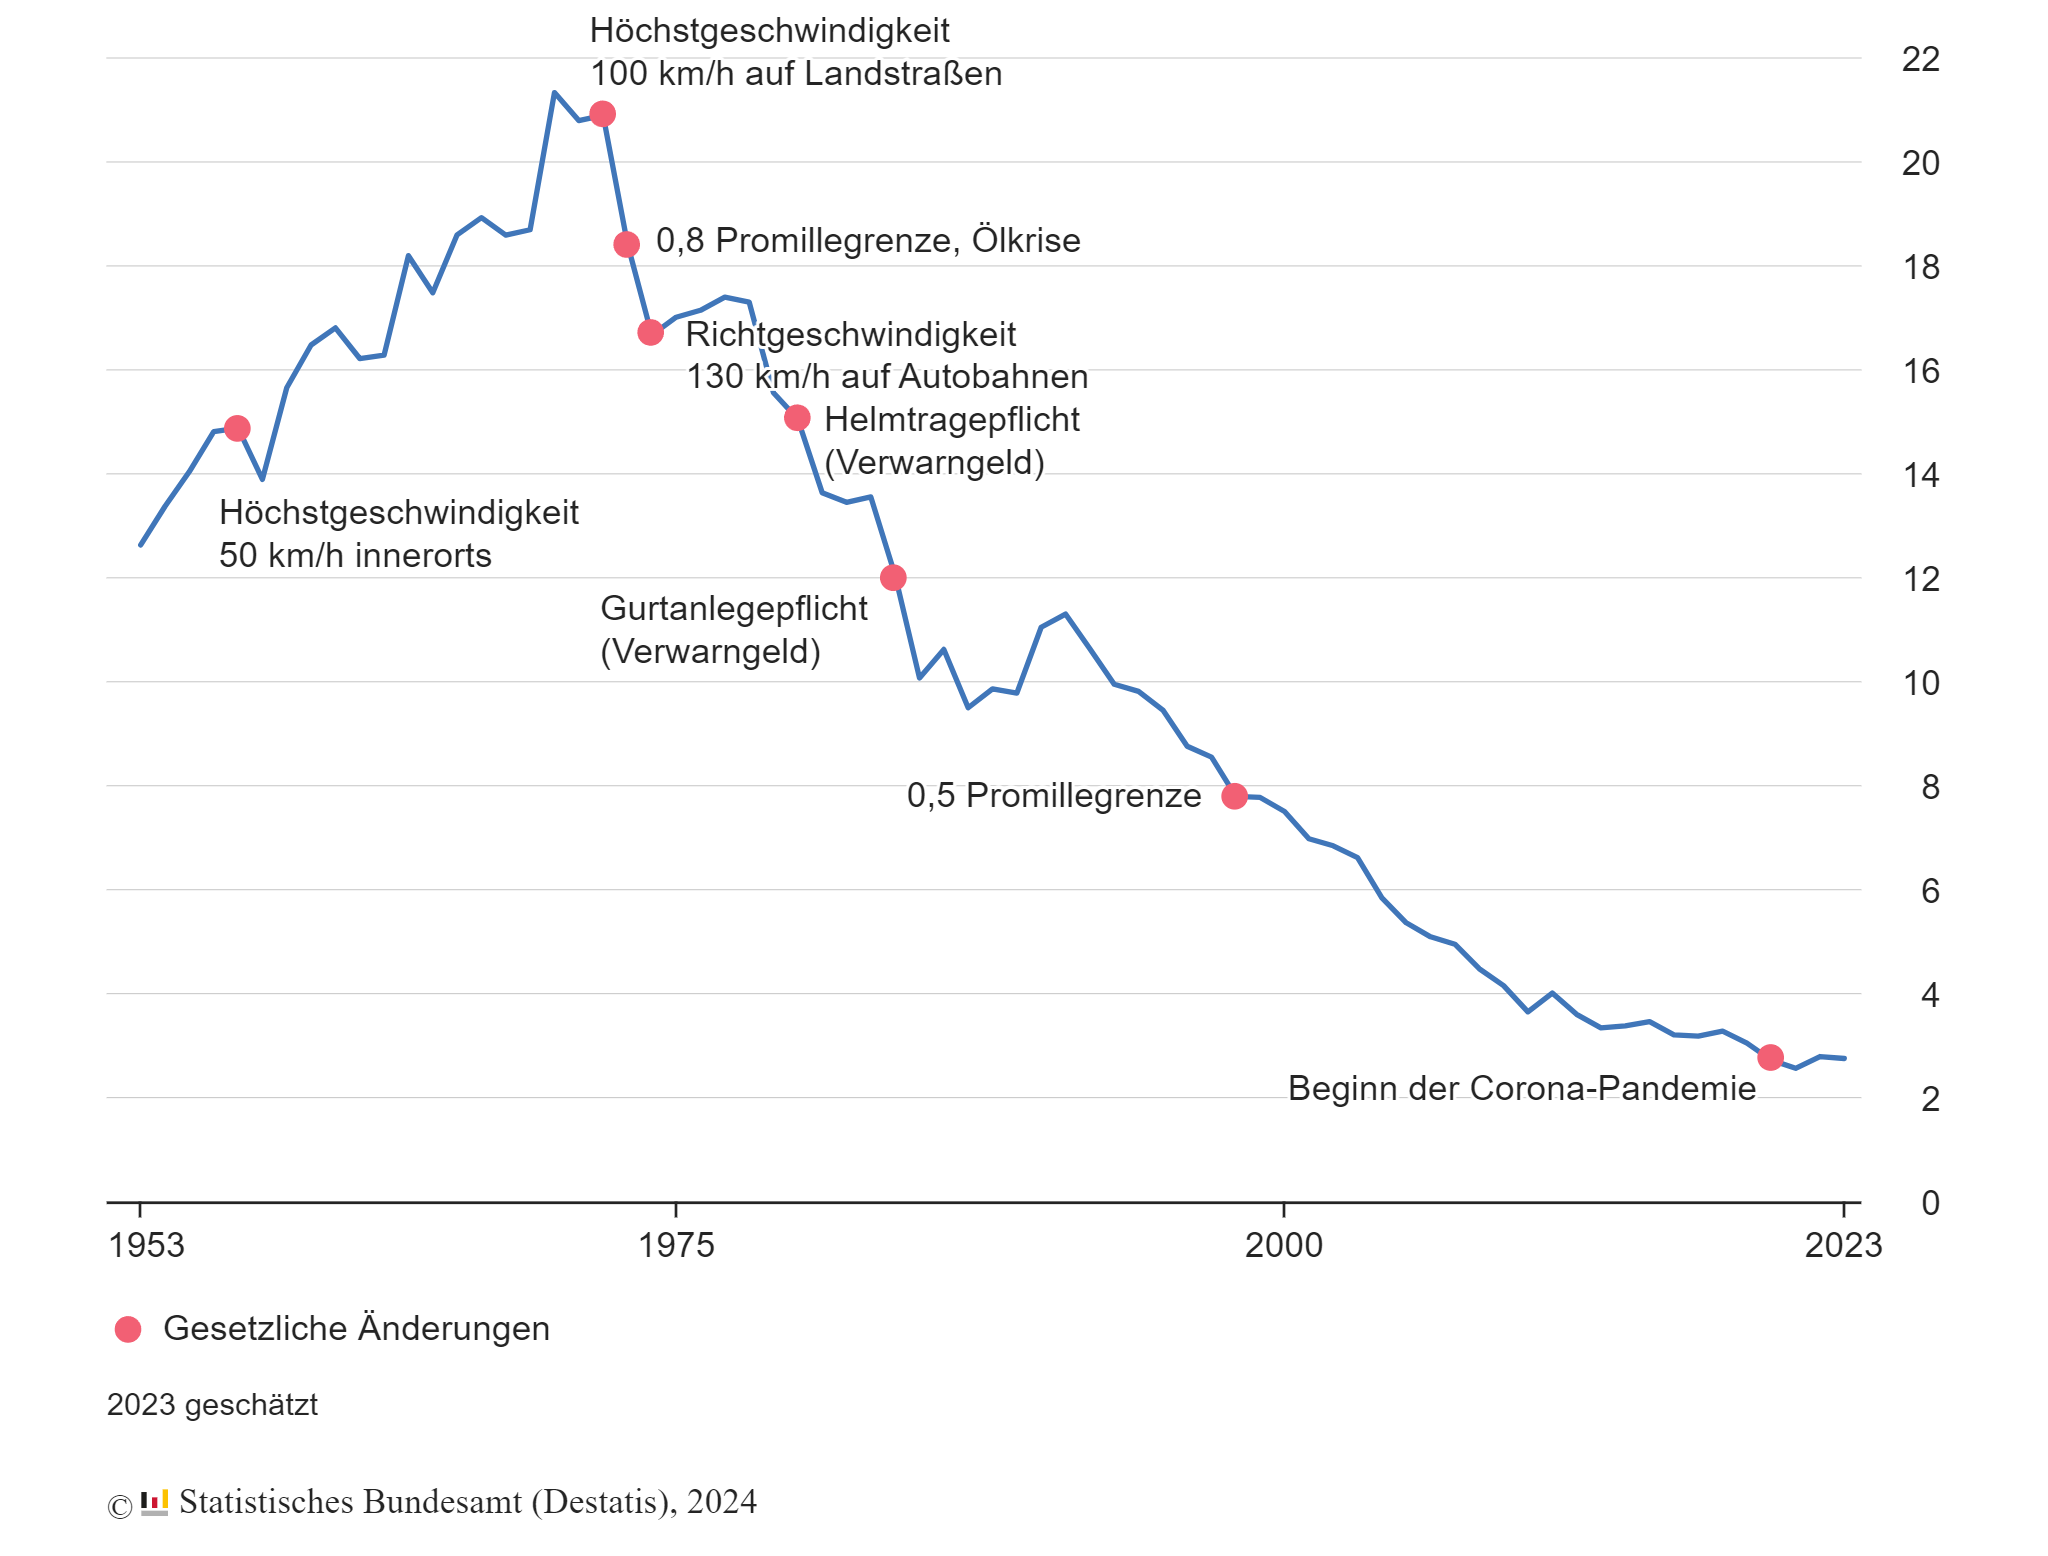
\includegraphics[width=0.9\textwidth]{figures/1_Einleitung/verkehrsunfaelle-getoetete-jahr.png}
    \caption{Bei Verkehrsunfällen Getötete pro Jahr in Tausend \cite{StBA2021}}
    \label{fig:Statistik_Tote}
\end{figure}
\noindent Im Jahr 2021 gab es über 250.000 Unfälle mit Personenschaden auf deutschen Straßen. In 88 \% der Fälle ist die Ursache auf ein Fehlverhalten der Fahrzeugführer zurückzuführen \cite{StBA2021}. Der Einsatz von automatisierten Fahrzeugen kann zu einem weiteren Rückgang der in Abbildung \ref{fig:Statistik_Tote} gezeigten Statistik führen, indem es den Fahrer durch Einsatz von intelligenten Assistenzsystemen unterstützt oder die menschliche Fehlerkomponente gänzlich beseitigt, indem ein Fahrzeug vollständig autonom fährt.

Um die Sicherheit der Fahrzeuge zu gewährleisten, muss sowohl das Gesamtsystem, als auch alle Teilsysteme intensiv getestet werden. Eines dieser Teilsysteme für das hochautomatisierte Fahren ist die Regelung der Längs- und Querführung des Fahrzeugs. Bei der IAV\footnote{\url{https://www.iav.com/}} geschieht dies durch einen modellprädiktiven Pfadfolgeregler.\bigskip

\noindent\textbf{Aufgabenstellung}\smallskip

\noindent Im Rahmen des Praktikums soll eine automatisierte Teststrategie für einen modellprädiktiven Pfadfolgeregler (engl. Model Predictive Pathfollowing Control, MPFC) konzeptioniert und implementiert werden.

Modellprädiktive Regler (engl. Model Predictive Control, MPC) eignen sich hervorragend für die Vorhersage und Regelung dynamischer Systeme, da sie auf Störungen im Betrieb gut reagieren können, weshalb sie in vielen Industriezweigen, einschließlich der Automobilindustrie, Anwendung finden \cite{adamy2014}. Im Bereich des hochautomatisierten Fahrens können mithilfe von MPC in Echtzeit Fahrentscheidungen, die sowohl sicherheits- als auch komfortrelevante Anforderungen erfüllen, getroffen werden. Um die Sicherheit und Zuverlässigkeit des Systems sicherzustellen, sollen realitätsnahe Fahrszenarien ermittelt und anhand von festgelegten Key Performance Indicators (KPIs) bewertet werden. Dieser Prozess soll automatisiert in einer CI Pipeline ablaufen.\medskip

\noindent Es sind die folgenden Teilaufgaben umzusetzen:
\begin{itemize}
    \item Konzeptentwicklung für das automatisierte, szenariobasierte Testen der MPFC unter Verwendung der bestehenden Simulationsumgebung
    \item Definition und Parametrierung geeigneter Fahrszenarien
    \item Definition von KPIs zur Beurteilung der Leistung der Regelung
    \item Einbindung in eine GitLab CI Pipeline
    \item Dokumentation der Ergebnisse
\end{itemize}
